\chapter{Curve ellittiche}

Abbiamo visto come, dato un reticolo $L \subseteq \bbC$, si possa costruire la funzione di Weierstrass associata $\wp_L (z)$, che insieme alla sua derivata $\wp'_L$ sono generatori del campo delle funzioni ellittiche, e inoltre soddisfano un'equazione del tipo $\wp'^2(z) = 4 \wp^3(z) - g_2 \wp(z) - g_3$ dove $g_2 = 60 G_2(L)$ e $g_3 = 140 G_3(L)$.

In generale, un'equazione cubica su $\bbP_2\bbC$ si dirà curva ellittica. Noi per ora ci occupiamo delle curve ellittiche che arrivano dai tori.

Prendiamo un toro $T=\quotient{\bbC}{L}$ con $L$ reticolo fissato, e sia $E: y^2 = A(x)=4x^3 - g_2 x - g_3$ la curva ellittica a lui associata; consideriamone poi la chiusura proiettiva $\ol{E} = E \cup \{ (0 : 1 : 0)\}$.

\begin{notazione}
  Con $\ol{E}(\bbK)$ si intendono i punti $\bbK$-razionali di $\ol{E}$, ovvero i punti di $\bbP^2 \bbC$ (facenti parte di $\ol{E}$) per le quali il rapporto tra le coordinate è un numero di $\bbK$, ovvero $\ol{E}(\bbK) = \{ (x : y : z) \in \ol{E} \mid \frac{x}{y}, \frac{y}{z} \in \bbK \}$
\end{notazione}

\section{Struttura di \sdR di una curva ellittica}

Per quanto visto nella prima parte, possiamo cercare un rivestimento $p: E(\bbC)\to\bbC$. In realtà quello che si riesce a fare è rivestire $D=\bbC\setminus\{z : A(z)=0\}$.

Prendiamo $(x_0,y_0)\in E(\bbC)$ con $y_0\neq0$; allora come mappa di rivestimento possiamo considerare la proiezione $\varphi(x,y)=x-x_0$ in un intorno. Infatti si ha $$ y=\sqrt{A(x)}=\sqrt{A(x_0)}\left(1+\frac{A(x)-A(x_0)}{A(x_0)} \right)^{\frac12} = y_0\left(1+\frac{A(x)-y_0^2}{y_0^2} \right)^{\frac12} = y_0s(y_0^2,x-x_0)$$
dove $s(y_0^2,x-x_0)$ è la serie di potenze in $x$ data dall'espansione della radice quadrata, che è localmente olomorfa.\\
Inoltre $\varphi^{-1}(u)=\{(u+x_0,y_0s(y_0^2,u)),(u+x_0,-y_0s(y_0^2,u))\}$ dove $y_0$ è una delle due radici quadrate di $A(x_0)$; è chiaro che fissando il segno ho un biolomorfismo locale.

Abbiamo dunque trovato un rivestimento $\pi: E(\bbC)\setminus\{y=0\}\to D$.

Per i punti in cui $y_0=0$, ovvero $x_0$ è radice del polinomio $A(x)$, possiamo fare un ragionamento analogo e invertire localmente: basta considerare la proiezione sull'altra componente, ovvero $\varphi(x,y)=y$. Infatti dato che $A(x_0)=0$ possiamo scrivere $A(x)=(x-x_0)A_1(x)$ con $A_1(x)$ non nullo in un intorno (dato che $A$ non ha radici multiple) e dunque ricavare $x-x_0=\frac{y^2}{A_1(x)}$ che è olomorfa.

\begin{proposizione}
    L'insieme dei punti della curva ellittica $\ol{E}(\bbC)$ è connesso
\end{proposizione}
\begin{proof}
    Consideriamo intanto $E(\bbC)$ (lo spazio dei punti affini).

    % $x \mapsto 4x^3 - g_2 x - g_3$

    Abbiamo appena visto che la funzione di proiezione $E(\bbC) \rar \bbC$ definita da $(x, y) \mapsto x$ diventa un rivestimento tolte le tre radici $\alpha, \beta, \gamma$ del polinomio $4x^3 - g_2 x - g_3$.

    \begin{center}
      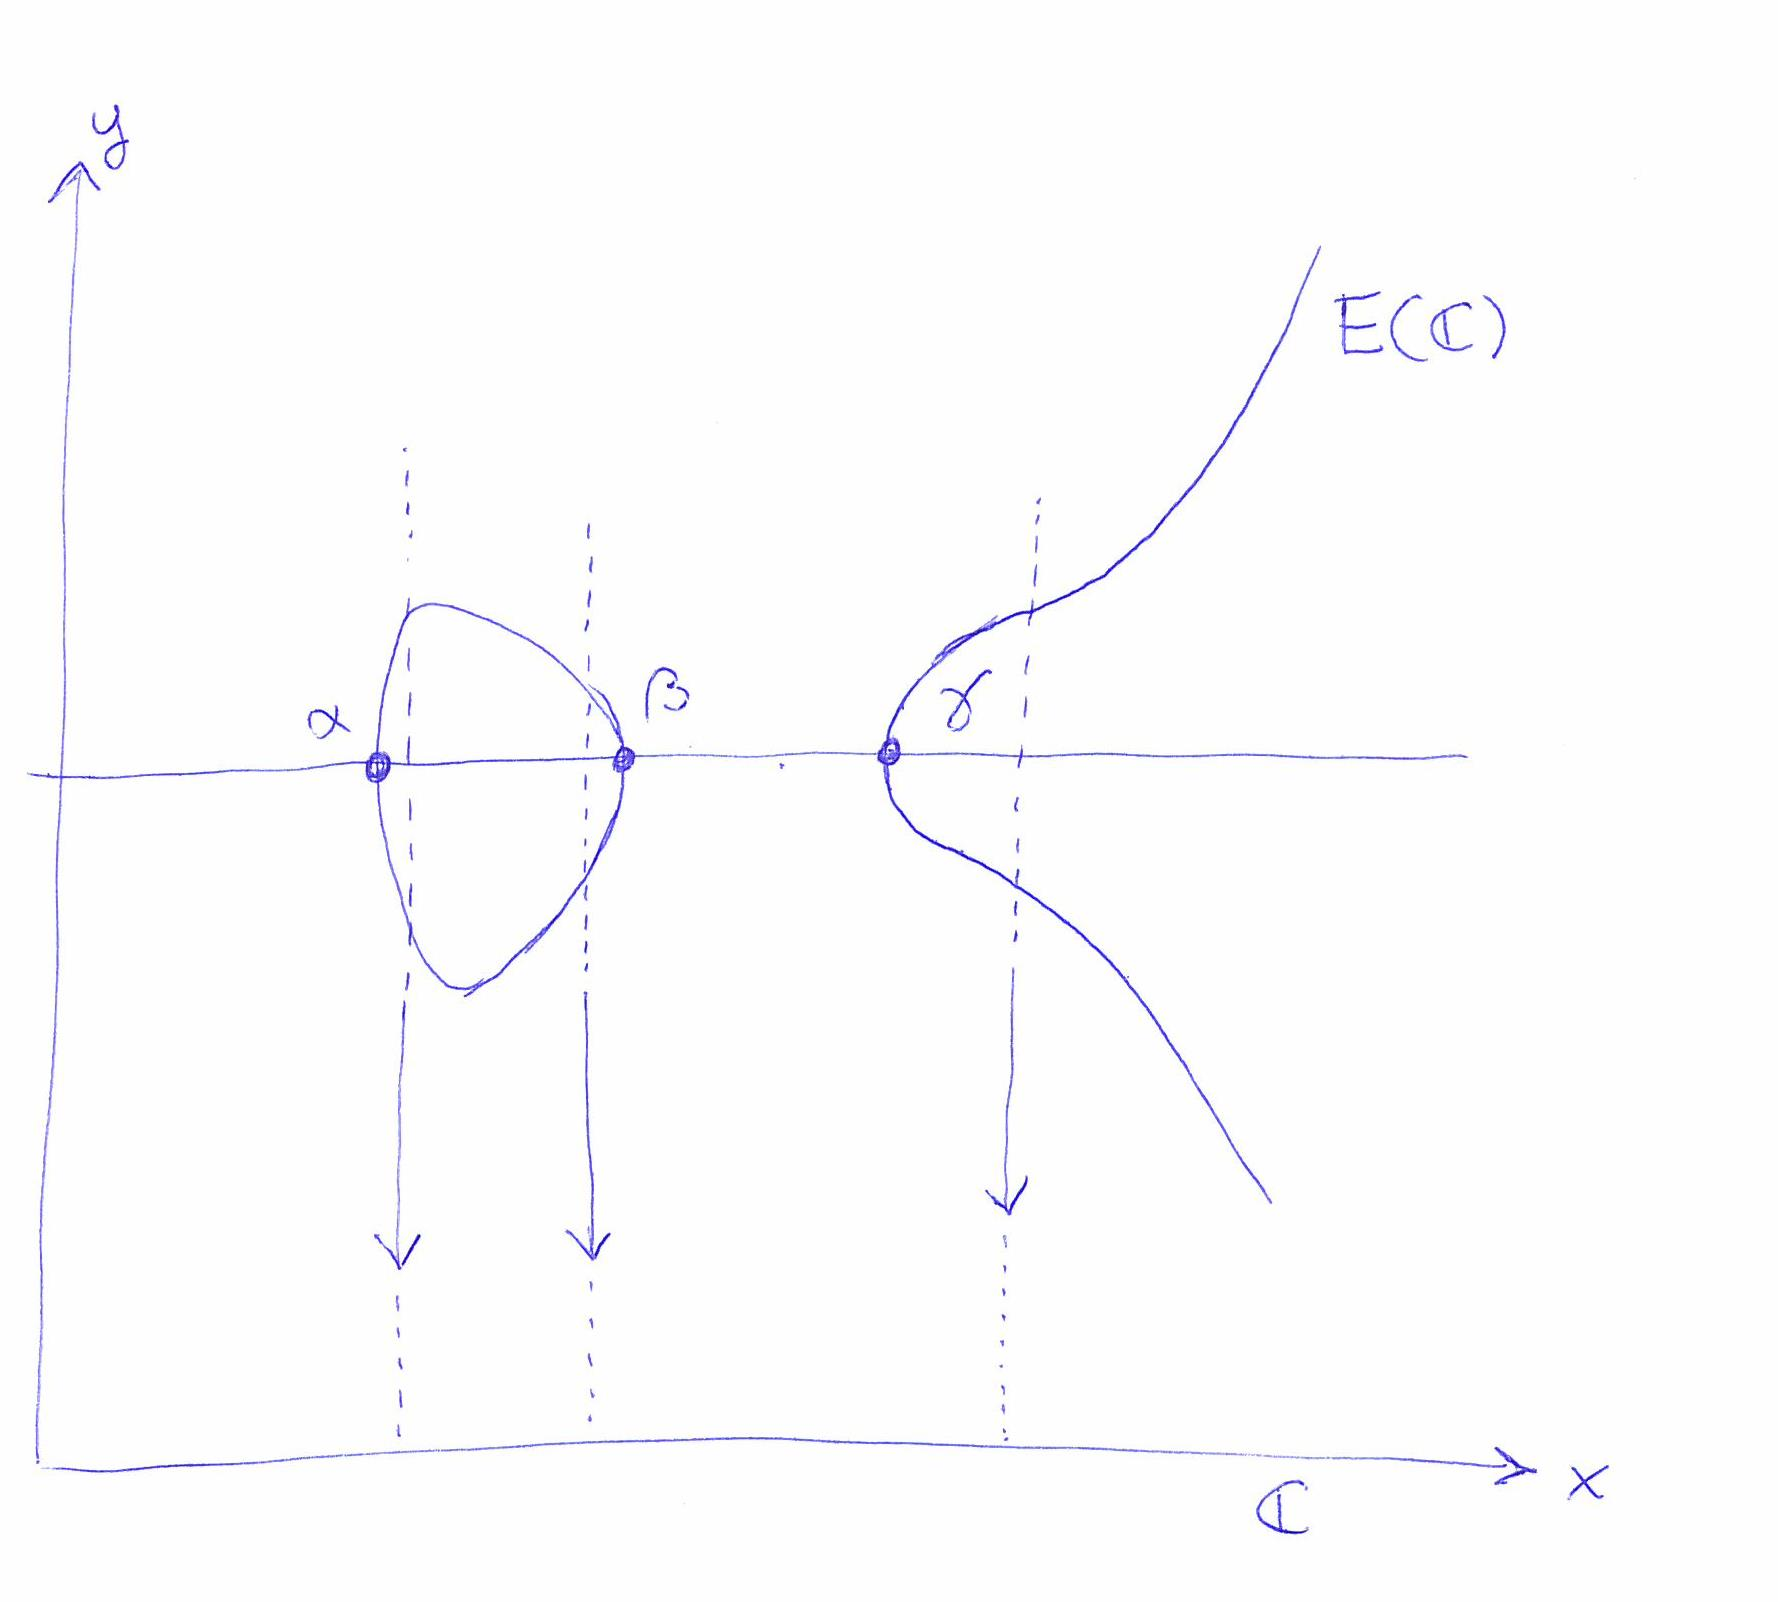
\includegraphics[width=8cm]{lezione-161128-fig1bis}
    \end{center}


    Ovviamente si ha che, avendo il rivestimento grado due, o è connesso, oppure ha due componenti connesse. Ora, se facciamo un cammino tra due punti $x_0$ ed $x_1$ del $\bbC$ ``che viene ricoperto'' posso sollevare il cammino, perché ho un rivestimento. Per mostrare la connessione del rivestimento basta quindi dimostrare che la fibra di $x_0 \neq \alpha,
    \beta, \gamma$ ``è connessa'', ovvero ho un cammino che connette i due elementi della fibra.

    \begin{center}
      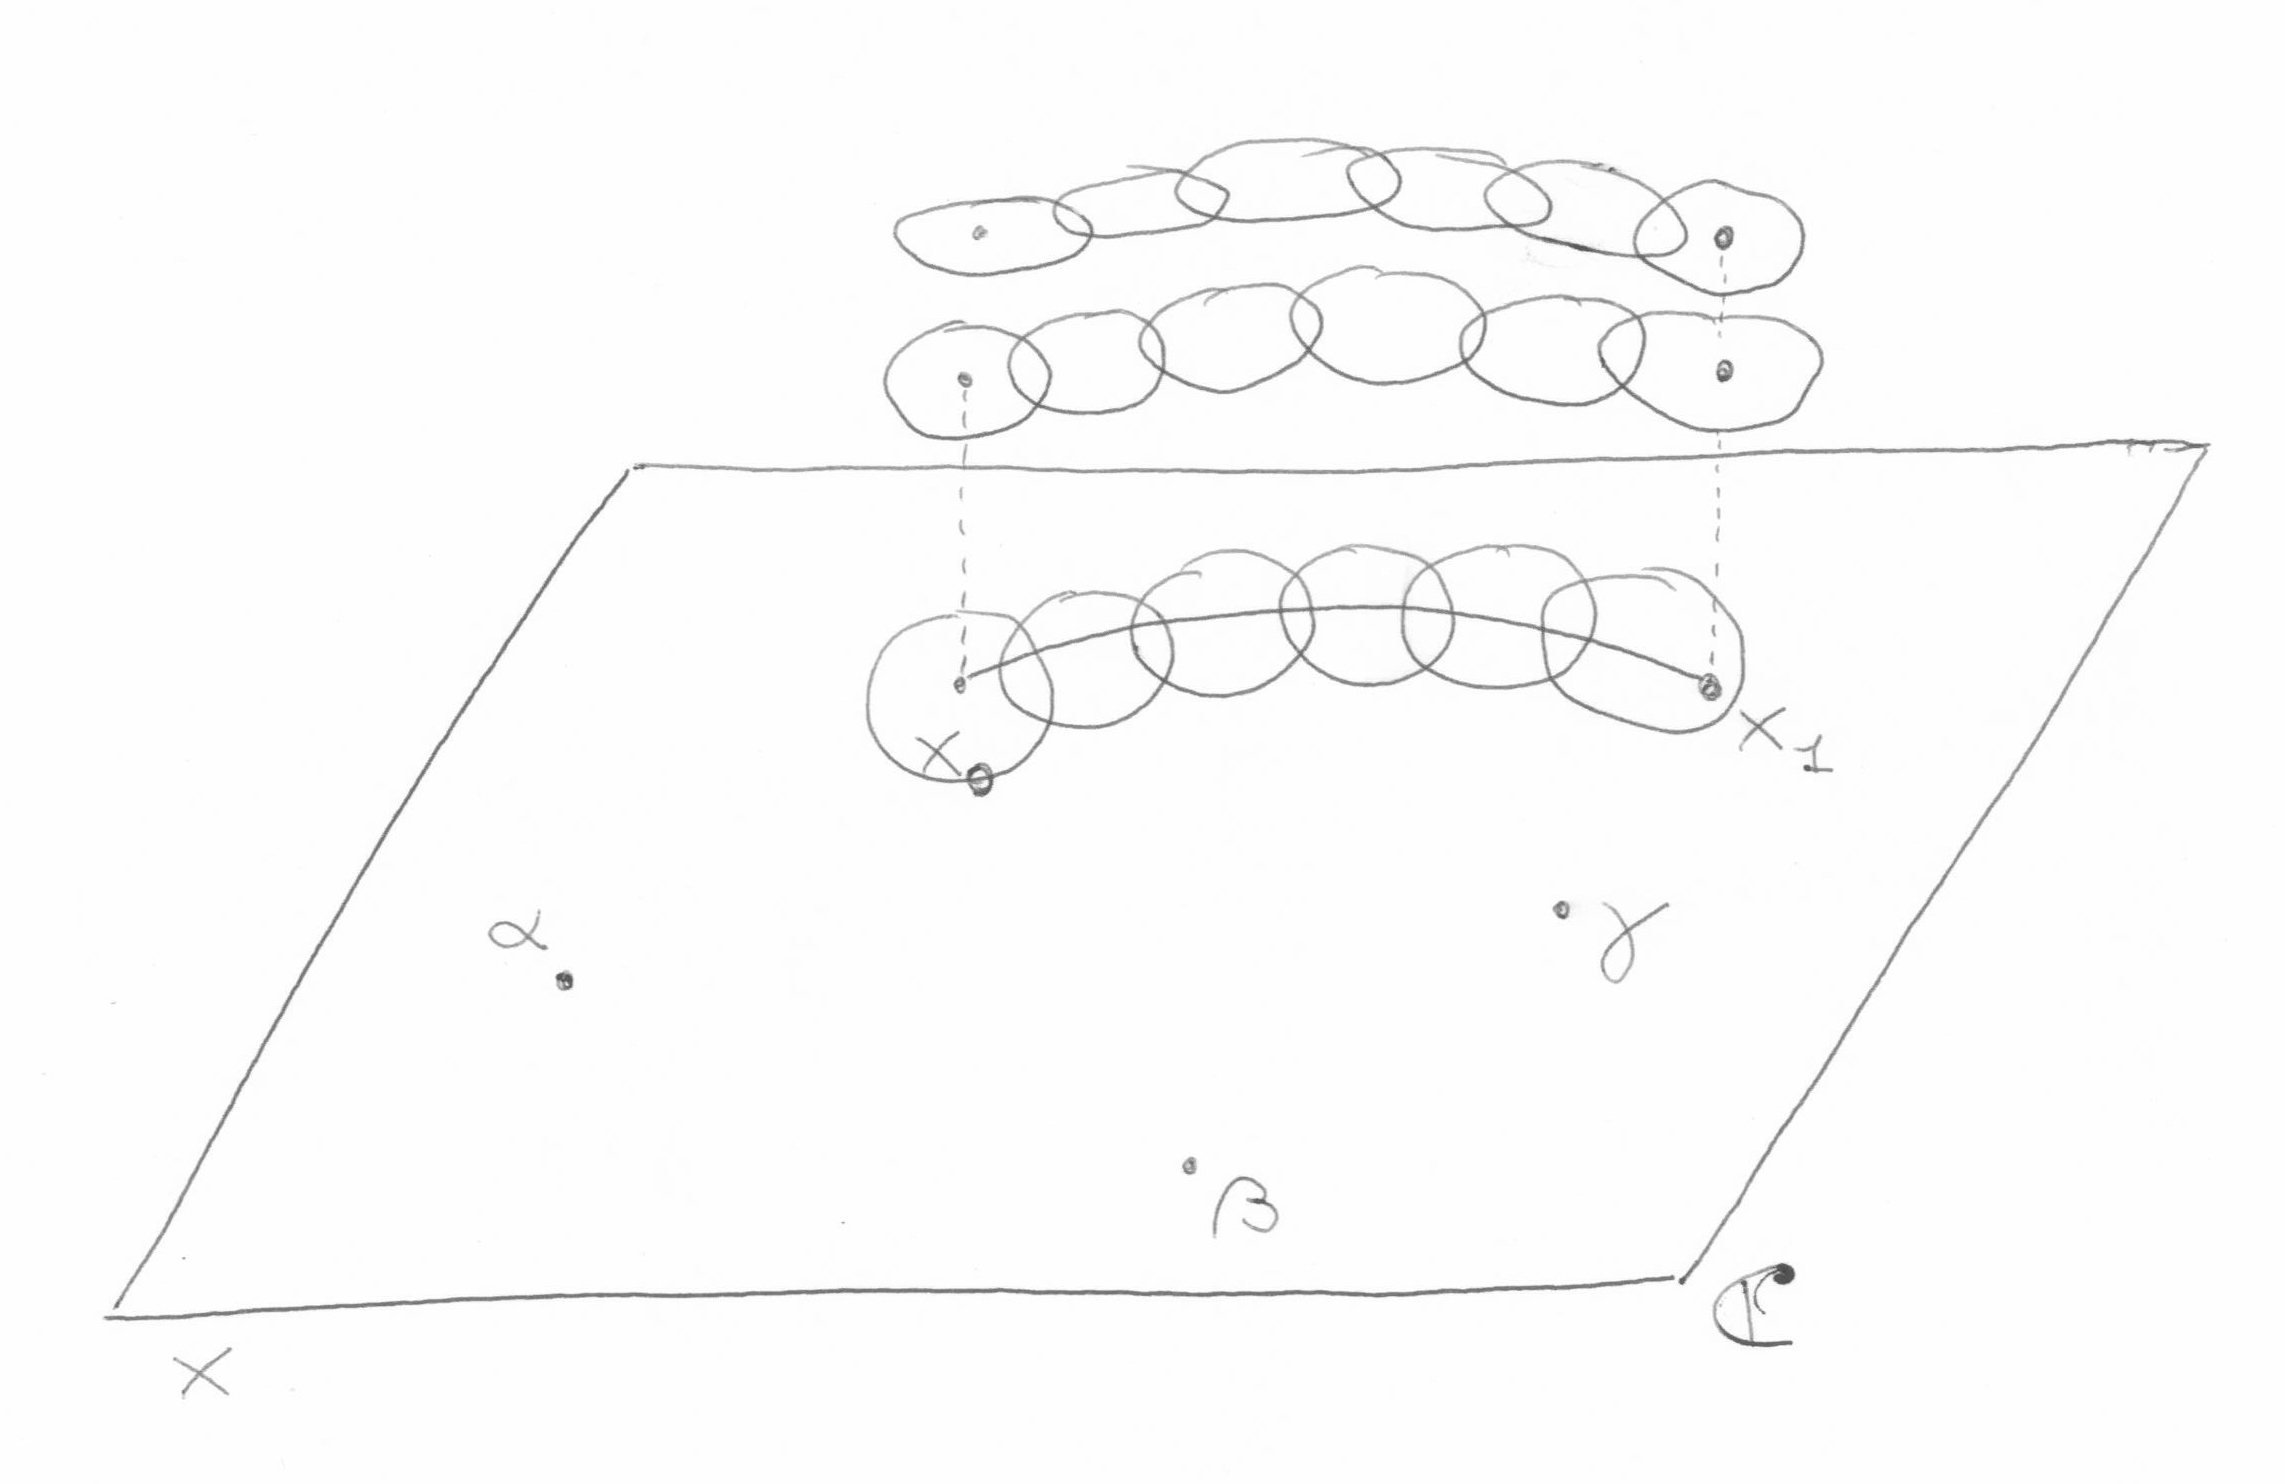
\includegraphics[width=8cm]{lezione-161128-fig2}
    \end{center}

    Ciò è molto semplice da fare con la radice quadrata: prendiamo infatti un punto $x_0$ vicino ad $\alpha$. Allora si ha che
    $\sqrt{f(x)} = (x - \alpha)^{\frac{1}{2}} \cdot g(x)$ con $g(x)$ olomorfa vicino ad $\alpha$ (poiché siamo lontani da $\beta$ e da $\gamma$)

    Scegliamo una determinazione della radice e facciamo un giro attorno ad $\alpha$ tornando sulla fibra di $x_0$ ma con valore del segno cambiato.

    \notamargine{In particolare si può scegliere un cerchio di raggio
      piccolo (cammino $t \mapsto x_0 + \rho e^{2\pi i t}$) e fare
      esplicitamente il conto ricordando che $z^\frac{1}{2}$ è definito con
      una determinazione di $e^{\log(\frac{1}{2} z)}$}
\end{proof}





\section{Un toro è biolomorfo alla sua curva ellittica}

Consideriamo la mappa $F: T = \quotient{\bbC}{L} \rar \ol{E}$ dal toro relativo al reticolo $L$ alla chiusura proiettiva della cubica. $F$ è definita da $z \mapsto (\wp(z) : \wp'(z) : 1)$ dove questa espressione ha senso. Quando invece $z$ è un polo di $\wp$, si può usare un'altra espressione per la mappa, ad esempio si può considerare l'espressione $\lbr{\frac{\wp(z)}{\wp'(z)} : 1 : \frac{1}{\wp'(z)}}$ dove se $\wp$ ha un polo doppio in $z$, $\wp'$ ha un polo triplo e quindi il rapporto ha ordine $1$ e possiamo definirlo uguale a $0$.\\
Notiamo che stiamo trattando $T$ come una varietà olomorfa e ciò che stiamo facendo è definire una mappa tra varietà su alcune carte.


\begin{proposizione}
  $F$ è una bigezione tra $T$ ed $\ol{E}(\bbC)$ (ed è olomorfa)
\end{proposizione}
\notamargine{Ricordiamo che tutte le funzioni meromorfe su $T$ sono
  $\bbC(\wp(z), \wp'(z))$, mentre le fuznioni meromorfe pari su $T$ sono
  esattamente $\bbC(\wp(z))$}
\begin{proof}
  Sia $p \in \ol{E}(\bbC)$. Distinguiamo in due casi:
  \begin{itemize}
  \item Se $p = (0 : 1 : 0)$ ok per costruzione (significa che la $\wp$
    ha un polo e quindi come unico punto abbiamo $z = 0 \in T$)
  \item Se $p \in E(\bbC)$ (nella parte affine della cubica) sia $p =
    (x_0, y_0)$

    Consideriamo allora $\wp(z) - x_0$ che è una funzione ellittica pari
    non costante che ha due zeri (con molteplicità). Se $z_0$ è uno zero
    lo è anche $- z_0$ (dove i punti si intendono sul
    toro). Distinguiamo in due casi a seconda della derivata nel punto:
    \begin{itemize}
    \item Se $\wp'(z_0) = 0$ allora $z_0$ è uno zero doppio e deve
      quindi coincidere con $-z_0$ sul toro, ovvero nel piano ho
      solamente quattro possibilità: sono la metà dei generatori del
      parallelogramma fondamentale del toro.

      \notamargine{Nella figura qui sotto è disegnato il
        parallelogramma fondamentale di un toro. Sono evidenziati con
        un pallino vuoto i punti che corrispondono alla metà dei
        generatori del parallelogrammo.

        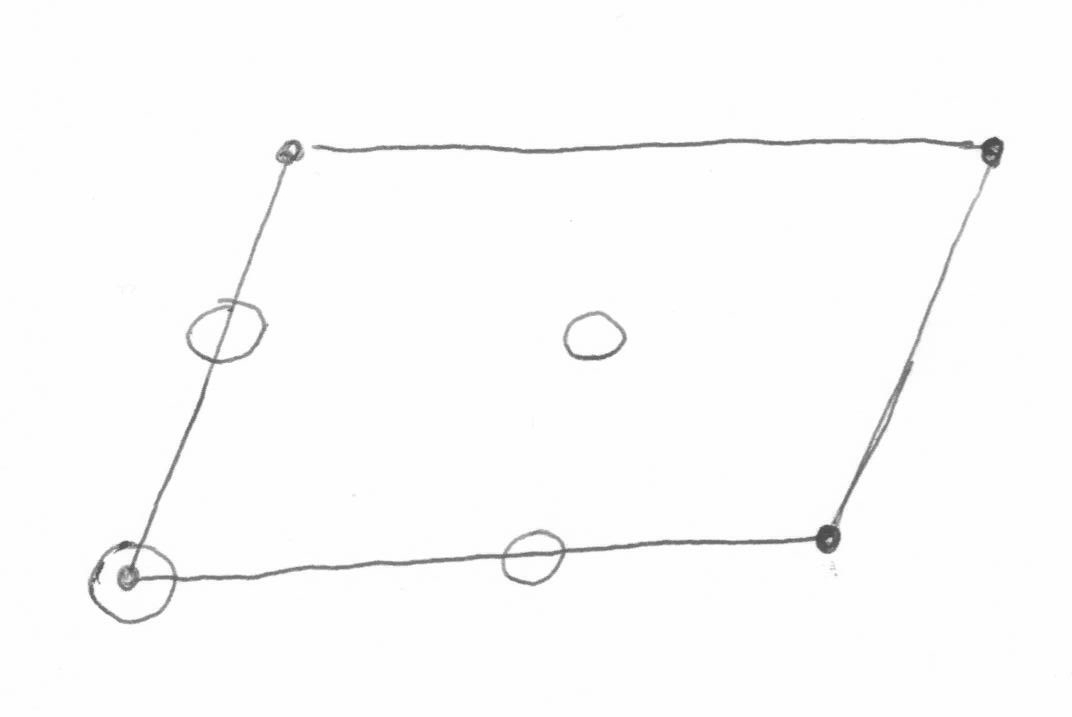
\includegraphics[width=3cm]{lezione-161128-fig1}}

      Allora si ha un solo punto tale che $4x_0^3 - g_2 x_0 - g_3 = 0 (=
      \wp'(z_0))$ e quindi anche questo caso è ok
    \item Se $\wp'(z_0) \neq 0$ allora si ha $z_0 \neq - z_0$ in $T$ e
      quindi $\wp'(z_0) = - \wp'(-z_0)$ poiché la $\wp'$ è
      dispari. Siamo allora nel caso $4x_0^3 - g_2 x_0 - g_3 = \alpha
      \neq 0$ e per avere $y = \pm \sqrt{\alpha}$ posso usare $z_0$ ed
      anche $-z_0$, ovvero ancora una volta la tesi è verificata.
    \end{itemize}
  \end{itemize}

  Per quanto riguarda l'olomorfia, basta aggiungere che la mappa fornita
  $z \mapsto (\wp(z) : \wp'(z) : 1)$ è ovviamente olomorfa tra $T$ e
  $\bbP^2 \bbC$
\end{proof}

\begin{osservazione}
  Notiamo però che se mi viene dato un polinomio di terzo grado nella
  forma $y^2 = 4x^3 - g_2 x - g_3$ non so ancora dire se venga da un
  toro oppure no. Se viene da un toro allora ho la corrispondenza
  biunivoca (proposizione precedente) $\sfrac{\bbC}{L} \leftrightarrow T$
\end{osservazione}

\begin{osservazione}
  Se abbiamo un polinomio in due variabili $f(x, y) = 0$ tale che
  $\nabla f$ non si annulli sul luogo di zeri di $f$ abbiamo una
  superficie di Riemman, ma non avevamo dimostrato (nel caso delle
  cubiche) la connessione, che in generale non è ovvia.

  Nel caso delle cubiche ciò segue dalla proposizione appena dimostrata.
\end{osservazione}


  Se ho una mappa $\phi: X \rar Y$, bigettiva e olomorfa tra superfici di Riemann, allora non è necessariamente biolomorfa.

  Infatti sia $C = \{ (x,y) \in \bbC^2 : y^2=x^3 \}$, e sia $\tilde C$ il suo completamento proiettivo. Allora detta $\phi: \bbP^1 \rar \tilde C$ la mappa $ (t : 1) \mapsto (t^2 : t^3 : 1)$ e $(1 : 0) \mapsto (0:1:0)$ questa è chiaramente bigettiva e olomorfa.

  Tuttavia l'inversa è data da $(x:y:1) \mapsto (\frac yx:1)$, che non è olomorfa in quanto il differenziale in $(0:0:1)$ è nullo (ma non è localmente costante).

  Il problema scaturisce dal fatto che il polinomio ha una radice doppia.

  Tuttavia se aggiungiamo che il differenziale sia full rank allora necessariamente deve essere biolomorfa.
  \begin{proof}
      Consideriamo il seguente diagramma:
      \[
      \begin{diagram}
          X & \rTo^\phi & Y \\
          \dTo>a & & \dTo>b \\
          \Omega_1 & \rTo^\psi & \Omega_2
      \end{diagram}
      \]

      $a, b$ sono le rispettive proiezioni in carta, quindi hanno differenziale full-rank. Segue che la composizione $\psi = b\circ \phi \circ a^{-1}$ ha anch'essa differenziale full-rank.
      Ora non capisco cosa stia cercando di scrivere formlmente, ma l'idea è che se ho il differenziale full-rank allora per il teorema di invertibilità locale posso trovare un'inversa differenziabile, e che soddisferà le condizioni per essere olomorfa. %TODO fare meglio%
  \end{proof}

  \begin{proposizione}
      La mappa di Weierstrass $F(z)=(\wp(z) : \wp'(z) : 1)$ è biolomorfa.
  \end{proposizione}
  \begin{proof}
      Abbiamo già visto che la $F$ è olomorfa e biiettiva, manca da dimostrare che l'inversa è olomorfa.
      Per questo mi basta guardare che il differenziale sia mai nullo. D'altra parte il differenziale della mappa di Weierstrass è $ (\wp'(z), \wp''(z))$ che non è mai nullo (Se abbiamo $\wp'(z_0) = \wp''(z_0) = 0$ vuol dire che $\wp'$ ha uno zero doppio in $z_0$, ma noi conosciamo già tutti gli zeri di $\wp'(z_0)$, che sono sui punti di $L/2$ diversi dall'origine).
  \end{proof}

  Grazie a questo possiamo dire che la curva ellittica ha la stessa struttura complessa del toro da cui proviene (se proviene effettivamente da un toro, cosa che si rivelerà vera).

  \begin{osservazione}
      Sul toro esiste una forma differenziale globale data da $dz$. Grazie alla mappa di Weierstrass, posso trasportarla sulla cubica e diventa $\frac{dx}y$, e segue che questa non ha poli, neanche all'infinito.\\
      Infatti nella parametrizzazione di Weierstrass, si ha che $x = \wp(z)$ e $y = \wp'(z)$. Allora, chiamata $g: E \rar \bbC$ l'inversa della parametrizzazione si ha che $g_*(\frac{dx}{y}) = \frac{d(\wp(z))}{\wp'(z)} = \frac{\wp'(z) dz}{\wp'(z)} = dz$

  \end{osservazione}

\section{Cubiche di $\bbP^2\bbC$}
Consideriamo tutte le cubiche in $\bbP^2\bbC$: esse sono definite da
un'equazione omogenea di grado tre $F(x, y, z) = 0$ con $F$
irriducibile. Mostreremo ora che la cubica è parametrizzabile se e solo
se è singolare.

\notamargine{Ricordiamo che per parametrizzazione intendiamo una
  isomorfismo birazionale con $\bbP^1$, ovvero una funzione razionale
  $f: \bbP^1 \rar E$ che si intende definita da quasi tutti i punti di
  $\bbP^1$ a quasi tutti i punti di $E$. (Quasi tutti significa tutti
  tranne al più un numero finito)}

\subsection{Caso singolare}
Sappiamo che esiste un punto singolare (ovvero che appartiene alla curva
e su cui tutte le derivate parziali dell'equazione definente la curva si
annullano, ovvero in cui la dimensione del tangente è due).

Allora, se intersechiamo la cubica con il fascio di rette passante per
il punto singolare otteniamo la parametrizzazione in termini del
``parametro angolare'' / tangente della retta per il punto (per esercizio
mostrare che ogni retta incontra esattamente un punto della chiusura
proiettiva della cubica e che, ovviamente, dato ogni punto della cubica
esiste una retta che passa per lui e per il punto singolare). La cubica
è quindi parametrizzabile.

Svolgiamo di seguito l'esercizio di cui sopra.
Supponiamo senza perdità di generalità che il punto singolare sia $(0,
0)$. Il fascio di rette si scrive allora come $y - \lambda x = 0$ con
$\lambda \in \bbP^1$. Cercare i punti comuni della cubica e della retta
significa sostituire nell'equazione della cubica $y = \lambda x$. A
questo punto otteniamo un polinomio di terzo grado che deve avere tre
radici, ma due ci sono già note ($x = 0$ è radice doppia). La terza
radice ora è funzione razionale dei coefficienti del polinomio, che
dipendono dal parametro $\lambda \in \bbP^1$.

\notamargine{Inoltre di punti singolari ne ha al più uno: se ve ne
  fossero due $p, q$ posso tracciare la retta passante per $p$ e per
  $q$, che intersecherebbe la cubica con molteplicità quattro.}

\subsection{Caso non singolare}
In ogni cubica c'è sempre un punto di flesso (ovvero dove l'hessiano si
annulla). Usando una proiettività si può mandare il flesso nel punto
all'infinito $(0 : 1 : 0)$.

\notamargine{L'Hessiano in questo caso è il determinante della matrice
  hessiana del polinomio che definisce la cubica, ovvero
  $\Det (\frac{\partial F}{\partial x_i \partial x_j})_{i, j = 1, 2, 3}$

  Il polinomio hessiano ha, per un facile conto, grado $3 (d-2)$, dove
  $d$ è il grado della curva $F$, oppure è identicamente nullo.
  Nel primo caso, per il teorema di Bèzout, esistono punti di $\bbP^2$
  su cui esso si annulla assieme all'equazione di $F$, ovvero esistono
  punti di $F$ di flesso (e sappiamo anche che sono $3 (d - 2) d$
  contati con molteplicità)}

Facendo i conti con il flesso all'infinito e con tangente al flesso la
retta $\{ z = 0 \}$ ottengo un'equazione simile a quella di Weierstrass
a cui si arriva con alcune manipolazioni algebriche:
$y^2 = 4 x^3 - a x - b$.

Se poi effettuiamo la trasformazione $x \mapsto \lambda^2 x$ e $y
\mapsto \lambda^3 y$ con $\lambda \neq 0$ allora si ottiene $y^2 = 4 x^3
- \frac{a}{\lambda^4} x - \frac{b}{\lambda^6}$.

Posso quindi scegliere $\lambda$ in modo da far scomparire un parametro.

\begin{osservazione}
  Non sappiamo ancora che ogni cubica viene da un toro, quindi non
  potevamo dire a priori che lo spazio delle cubiche ha un solo
  parametro.
\end{osservazione}

Che succede se al posto di un reticolo $L$ ne prendiamo uno omotetico
$\lambda L$ con $\lambda \in \bbC^*$? Le funzioni $g_2$ e $g_3$ si
trasformano nel seguente modo:
$ g_2 \mapsto \frac{g_2}{\lambda^4} ,\quad g_3 \mapsto
\frac{g_3}{\lambda^6}$ e quindi l'equazione della cubica diventa:
$E_{\lambda L}: y^2 = 4x^3 - \frac{g_2}{\lambda^4} x -
\frac{g_3}{\lambda^6}$

Quali sono le funzioni razionali di $a$ e di $b$ che rimangono
invarianti per trasformazioni omotetiche? Sicuramente vi è
$\frac{a^3}{b^2}$.
\notamargine{Per esercizio si può dimostrare che ogni funzione razionale
  invariante per omotetia di $a$ e di $b$ si scrive come funzione
  razionale di $\frac{a^3}{b^2}$}

Dato un reticolo $L$, lo scriviamo come $\bbZ \tau + \bbZ$ con $\tau \in
\cH$ (semipiano superiore) a meno di rotomotetie del piano.

\begin{proposizione}
  $\frac{g_2^3}{g_3^2}$ è una funzione di $\tau$ non costante e meromorfa
\end{proposizione}

Per quanto riguarda la meromorfia, si può notare che, definita la somma
$$S_n = \sum_{(r, s) \in \bbZ^2 \setminus \{(0, 0)\}} \frac{1}{(r \tau
  + s)^n}$$ essa converge per $n \ge 2$ e definisce una funzione olomorfa
di $\tau$. Segue quindi che, se $S_3$ non è identicamente nulla, si ha
che $\frac{g_2^3}{g_3^2} = \frac{S_2^3(\tau)}{S_3^2(\tau)}$ per
definizione e quindi la succitata funzione è meromorfa.

\notamargine{Per verificare la convergenza assoluta della sommatoria per
  $n > 2$ si può maggiorare la serie dei valori assoluti con l'opportuno
  integrale in due variabili. Per il caso $n=2$ non saprei...}

Inoltre, se trovassimo due reticoli $L_1$ ed $L_2$ in cui valga
rispettivamente
$$g_3(L_1) = 0, g_2(L_1) \neq 0$$
$$g_2(L_2) = 0, g_3(L_2) \neq 0$$
ne seguirebbe che la funzione non è costante.

Si possono a tal proposito considerare i reticoli $\tau = i$ e
$\tau = \zeta_3$:
\begin{itemize}
\item ($\tau = i$) Sia $L_1 = \bbZ[i]$. Allora si nota che $i L_1 = L_1$
  e quindi si ha $g_2(i L_1) = g_2(L_1)$ e per omogeneità
  $g_3(L_1) = g_3(i L_1) = i^{-6} g_3(L_1)$ da cui segue $g_3(L_1) = 0$.

  Inoltre $g_2 \neq 0$, altrimenti il polinomio definente avrebbe radici
  multiple (segue direttamente dall'equazione del polinomio).

\item ($\tau = \zeta_3$) Sia $L_2 = \bbZ[\zeta_3]$ e notiamo che
  $\zeta_3 L_2 = L_2$ che implica $g_2(L_2) = g_2(\zeta_3 L_2) =
  \zeta_3^4 g_2(L_2) = \zeta_3 g_2(L_2)$ e quindi $g_2(L_2) = 0$
\end{itemize}





	\section{Discriminante e invariante $j$}

	Ricordiamo che per una cubica del tipo $y^2=p(x)$ la non singolarità equivale all'assenza di radici multiple. Un modo rapido per vedere se un polinomio ha radici multiple è definire il discriminante.

	Sia quindi $f(t)$ un polinomio con radici $\alpha_i$ (eventualmente ripetute), definiamo $\Delta(f)=\prod_{i<j} (\alpha_i - \alpha_j)^2$. Questo è simmetrico nelle radici pertanto lo posso scrivere come un polinomio a coefficienti interi nei coefficienti di $f$.
    \notamargine{Possiamo anche definire $\Delta(f)=\Ris(f,f')$ il risultante tra $f$ e la sua derivata.}

	Se $f=ax^2+bx+c$, allora $\Delta(a,b,c)= b^2-4ac$.

    Calcoliamolo ora per $\deg f=3$. Prendo $f(t)=t^3+At+B$. Essendo $\Delta$ di grado 6 nei coefficienti, deve essere combinazione linerare di $A^3$ e $B^2$. Ora mettendomi nel caso particolare $A=0,B=-1$ e nel caso $B=0$ posso agilmente scoprire che
	\[
		\Delta(A,B)=-4A^3-27B^2
	\]


	Sappiamo che ogni cubica non singolare è isomorfa a $y^2=x^3-ax-b$ mediante trasformazioni affini.

	Considero il parametro $\frac{a^3}{b^2}$. Sappiamo che è invariante per le omotetie del tipo $x\mapsto \lambda^2x, y\mapsto\lambda^3y$. Ho però il problema che esso non è definito per $b=0$.

	Utilizzo quindi il discriminante. So che dato che il polinomio non ha radici multiple, il discriminante sarà non nullo: sfrutto questa informazione per considerare come parametro una funzione che dipenda solo da $\frac{a^3}{b^2}$ che abbia il discriminante come denominatore. Uso quindi

	\[
		j = c \cdot \frac {a^3}{a^3-27b^2}
	\]

	Convenzionalmente, invece dell'ovvia $c=1$ si pone $c=1728$ per qualche oscuro motivo.

	Mostriamo ora che una cubica proveniente da un toro non ha radici multiple.

	\begin{proof}
		Sappiamo che
		\[
			\wp'(z)^2=4\wp(z)^3-g_2\wp(z)-g_3 = 4(\wp(z)-e_1)(\wp(z)-e_2)(\wp(z)-e_3)
		\]

		Quindi $\wp(z_0)=e_i \Rar\wp'(z_0)=0$.
		Se $L=\bbZ\omega_1 + \bbZ\omega_2$, allora $\wp'(z)$ si deve annullare su tutti i punti di $\frac L2$: infatti se $l \in \frac L2$ allora $l \equiv -l \pmod L$, e dato che $\wp'(z)$ è dispari ho che
		\[
			\wp(l) = \wp(-l) = -\wp(l)
		\]

		Visto sul toro, $\wp'(z)$ si annulla in quattro punti.

		E invece no! Ho mentito. Nell'origine non si annulla, c'è un polo. Dato che $\wp'(z)$ ha esattamente un polo di ordine tre, allora ho trovato tutti gli zeri, che sono $\frac{\omega_1}2, \frac{\omega_2}2, \frac{\omega_1+\omega_2}2$.

		%TODO manca da dire perché sono davvero distinte, che non sto ben capendo
                % Sono distinte perché se ho om1/2 = om2/2 ==> om1 = om2 assurdo perché i generatori del reticolo sono distinti
                % Il caso om1/2 = (om1+om2)/2 ==> om2 = 0 assurdo perché so che devono generare un reticolo di rango due

	\end{proof}

	Ora vediamo che tori con la stessa $j$ sono omotetici.

	\begin{proof}
          Suppongo che $T, T'$ abbiano la stessa $j$. Allora ho $\frac{a^3}{b^2}=\frac{a'^3}{b'^2}$. Quindi se con un omotetia faccio in modo che $a$ venga mandato in $a'$, allora sicuramente $b$ viene mandato in $b'$ oppure in $-b'$.

          Osserviamo che le due cubiche che in forma normale di Weierstrass hanno come parametri $a, b$ e $a, -b$ sono in realtà la stessa curva. Infatti applicando la trasformazione $x' = -x$, $y' = iy$ si ha $y^2 = 4x^3 - ax - b \mapsto - y'^2 = - 4x'^3 + ax - b$ che coincide con la forma $y'^2 = 4x'^3 - ax - (-b)$.

          Quindi sia $T$ che $T'$ sono biolomorfi alla stessa curva, quindi sono biolomorfi tra loro e dunque omotetici.
	\end{proof}

	\begin{osservazione}
		$j(\tau)$ è una funzione non costante e olomorfa. Vedremo anche che è suriettiva.
	\end{osservazione}
